% Created by tikzDevice version 0.12.3.1 on 2022-09-02 10:41:13
% !TEX encoding = UTF-8 Unicode
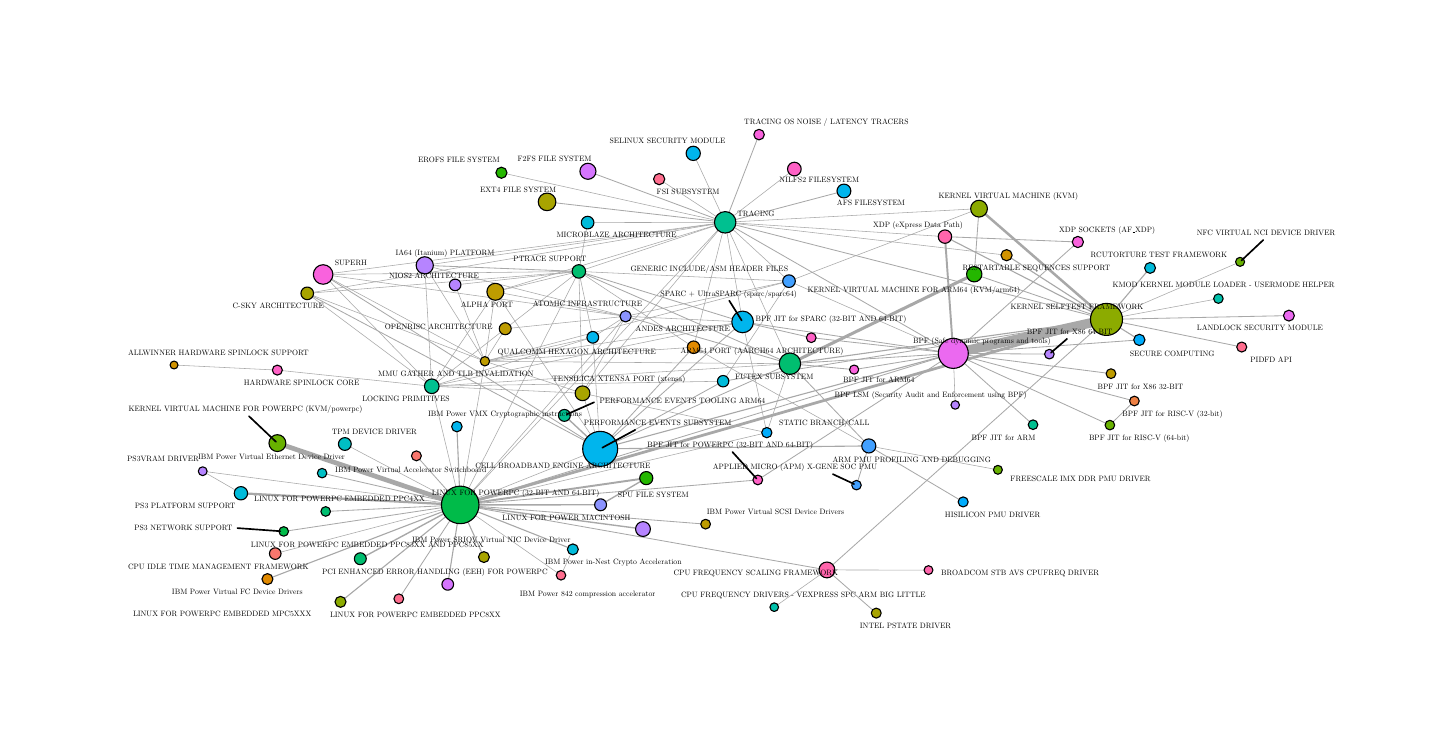
\begin{tikzpicture}[x=1pt,y=1pt]
\definecolor{fillColor}{RGB}{255,255,255}
\path[use as bounding box,fill=fillColor,fill opacity=0.00] (0,0) rectangle (505.89,252.94);
\begin{scope}
\path[clip] (  0.00,  0.00) rectangle (505.89,252.94);
\definecolor{fillColor}{RGB}{255,255,255}

\path[fill=fillColor] (  0.00,  0.00) rectangle (505.89,252.94);
\end{scope}
\begin{scope}
\path[clip] ( 32.75, 32.75) rectangle (475.89,222.94);
\definecolor{drawColor}{gray}{0.66}

\path[draw=drawColor,line width= 0.3pt,line join=round] (294.95,193.92) -- (252.04,182.60);

\path[draw=drawColor,line width= 0.2pt,line join=round] ( 52.89,131.04) -- ( 90.22,129.20);

\path[draw=drawColor,line width= 0.2pt,line join=round] (169.00,157.50) -- (216.05,148.64);

\path[draw=drawColor,line width= 0.2pt,line join=round] (169.00,157.50) -- (146.02,123.36);

\path[draw=drawColor,line width= 0.2pt,line join=round] (169.00,157.50) -- (165.22,132.40);

\path[draw=drawColor,line width= 0.2pt,line join=round] (169.00,157.50) -- (206.87,100.74);

\path[draw=drawColor,line width= 0.2pt,line join=round] (169.00,157.50) -- (199.16,164.86);

\path[draw=drawColor,line width= 0.2pt,line join=round] (169.00,157.50) -- (252.04,182.60);

\path[draw=drawColor,line width= 0.2pt,line join=round] (240.63,137.46) -- (303.94,101.80);

\path[draw=drawColor,line width= 0.2pt,line join=round] (240.63,137.46) -- (165.22,132.40);

\path[draw=drawColor,line width= 0.3pt,line join=round] (240.63,137.46) -- (206.87,100.74);

\path[draw=drawColor,line width= 0.2pt,line join=round] (240.63,137.46) -- (199.16,164.86);

\path[draw=drawColor,line width= 0.2pt,line join=round] (240.63,137.46) -- (252.04,182.60);

\path[draw=drawColor,line width= 0.3pt,line join=round] (299.49, 87.63) -- (303.94,101.80);

\path[draw=drawColor,line width= 0.3pt,line join=round] (303.94,101.80) -- (275.44,131.50);

\path[draw=drawColor,line width= 0.2pt,line join=round] (303.94,101.80) -- (350.59, 93.17);

\path[draw=drawColor,line width= 0.3pt,line join=round] (303.94,101.80) -- (338.04, 81.57);

\path[draw=drawColor,line width= 0.4pt,line join=round] (303.94,101.80) -- (206.87,100.74);

\path[draw=drawColor,line width= 0.3pt,line join=round] (275.44,131.50) -- (216.05,148.64);

\path[draw=drawColor,line width= 0.3pt,line join=round] (275.44,131.50) -- (334.47,135.24);

\path[draw=drawColor,line width= 0.3pt,line join=round] (275.44,131.50) -- (298.64,129.38);

\path[draw=drawColor,line width= 0.4pt,line join=round] (275.44,131.50) -- (389.83,147.52);

\path[draw=drawColor,line width= 1.1pt,line join=round] (275.44,131.50) -- (342.04,163.85);

\path[draw=drawColor,line width= 0.2pt,line join=round] (275.44,131.50) -- (146.02,123.36);

\path[draw=drawColor,line width= 0.2pt,line join=round] (275.44,131.50) -- (165.22,132.40);

\path[draw=drawColor,line width= 0.3pt,line join=round] (275.44,131.50) -- (206.87,100.74);

\path[draw=drawColor,line width= 0.3pt,line join=round] (275.44,131.50) -- (199.16,164.86);

\path[draw=drawColor,line width= 0.2pt,line join=round] (275.44,131.50) -- (267.09,106.61);

\path[draw=drawColor,line width= 0.2pt,line join=round] (275.44,131.50) -- (252.04,182.60);

\path[draw=drawColor,line width= 0.2pt,line join=round] (216.05,148.64) -- (275.11,161.34);

\path[draw=drawColor,line width= 0.2pt,line join=round] (216.05,148.64) -- (143.48,167.05);

\path[draw=drawColor,line width= 0.2pt,line join=round] (216.05,148.64) -- (156.30, 80.49);

\path[draw=drawColor,line width= 0.2pt,line join=round] (216.05,148.64) -- (172.57,144.15);

\path[draw=drawColor,line width= 0.2pt,line join=round] (216.05,148.64) -- (204.21,141.05);

\path[draw=drawColor,line width= 0.2pt,line join=round] (216.05,148.64) -- (258.34,146.61);

\path[draw=drawColor,line width= 0.2pt,line join=round] (216.05,148.64) -- (106.76,163.75);

\path[draw=drawColor,line width= 0.2pt,line join=round] (216.05,148.64) -- (200.50,120.83);

\path[draw=drawColor,line width= 0.3pt,line join=round] (334.47,135.24) -- (363.28,109.47);

\path[draw=drawColor,line width= 0.3pt,line join=round] (334.47,135.24) -- (298.64,129.38);

\path[draw=drawColor,line width= 0.3pt,line join=round] (334.47,135.24) -- (263.82, 89.51);

\path[draw=drawColor,line width= 0.3pt,line join=round] (334.47,135.24) -- (399.91,118.03);

\path[draw=drawColor,line width= 0.3pt,line join=round] (334.47,135.24) -- (391.05,109.33);

\path[draw=drawColor,line width= 0.3pt,line join=round] (334.47,135.24) -- (283.15,140.91);

\path[draw=drawColor,line width= 0.3pt,line join=round] (334.47,135.24) -- (391.45,127.92);

\path[draw=drawColor,line width= 0.3pt,line join=round] (334.47,135.24) -- (369.19,134.97);

\path[draw=drawColor,line width= 0.2pt,line join=round] (334.47,135.24) -- (335.17,116.60);

\path[draw=drawColor,line width= 0.2pt,line join=round] (334.47,135.24) -- (275.11,161.34);

\path[draw=drawColor,line width= 3.4pt,line join=round] (334.47,135.24) -- (389.83,147.52);

\path[draw=drawColor,line width= 0.3pt,line join=round] (334.47,135.24) -- (156.30, 80.49);

\path[draw=drawColor,line width= 0.4pt,line join=round] (334.47,135.24) -- (206.87,100.74);

\path[draw=drawColor,line width= 0.3pt,line join=round] (334.47,135.24) -- (401.70,140.12);

\path[draw=drawColor,line width= 0.3pt,line join=round] (334.47,135.24) -- (258.34,146.61);

\path[draw=drawColor,line width= 0.3pt,line join=round] (334.47,135.24) -- (252.04,182.60);

\path[draw=drawColor,line width= 0.7pt,line join=round] (334.47,135.24) -- (331.46,177.43);

\path[draw=drawColor,line width= 0.3pt,line join=round] (334.47,135.24) -- (379.48,175.49);

\path[draw=drawColor,line width= 0.3pt,line join=round] (263.82, 89.51) -- (156.30, 80.49);

\path[draw=drawColor,line width= 0.3pt,line join=round] (399.91,118.03) -- (391.05,109.33);

\path[draw=drawColor,line width= 0.3pt,line join=round] (283.15,140.91) -- (258.34,146.61);

\path[draw=drawColor,line width= 0.2pt,line join=round] (325.51, 56.93) -- (288.81, 56.99);

\path[draw=drawColor,line width= 0.2pt,line join=round] (101.02,156.93) -- (146.02,123.36);

\path[draw=drawColor,line width= 0.2pt,line join=round] (101.02,156.93) -- (165.22,132.40);

\path[draw=drawColor,line width= 0.3pt,line join=round] (101.02,156.93) -- (206.87,100.74);

\path[draw=drawColor,line width= 0.2pt,line join=round] (101.02,156.93) -- (199.16,164.86);

\path[draw=drawColor,line width= 0.2pt,line join=round] (101.02,156.93) -- (252.04,182.60);

\path[draw=drawColor,line width= 0.7pt,line join=round] (223.53, 90.17) -- (156.30, 80.49);

\path[draw=drawColor,line width= 0.5pt,line join=round] (223.53, 90.17) -- (207.02, 80.54);

\path[draw=drawColor,line width= 0.2pt,line join=round] (269.77, 43.54) -- (288.81, 56.99);

\path[draw=drawColor,line width= 0.3pt,line join=round] (288.81, 56.99) -- (306.63, 41.40);

\path[draw=drawColor,line width= 0.3pt,line join=round] (288.81, 56.99) -- (389.83,147.52);

\path[draw=drawColor,line width= 0.3pt,line join=round] (288.81, 56.99) -- (156.30, 80.49);

\path[draw=drawColor,line width= 0.2pt,line join=round] ( 89.46, 62.90) -- (156.30, 80.49);

\path[draw=drawColor,line width= 0.2pt,line join=round] (171.19,200.52) -- (252.04,182.60);

\path[draw=drawColor,line width= 0.3pt,line join=round] (187.68,189.99) -- (252.04,182.60);

\path[draw=drawColor,line width= 0.3pt,line join=round] (202.45,201.04) -- (252.04,182.60);

\path[draw=drawColor,line width= 0.2pt,line join=round] (228.19,198.21) -- (252.04,182.60);

\path[draw=drawColor,line width= 0.2pt,line join=round] (251.30,125.19) -- (275.11,161.34);

\path[draw=drawColor,line width= 0.3pt,line join=round] (251.30,125.19) -- (389.83,147.52);

\path[draw=drawColor,line width= 0.2pt,line join=round] (251.30,125.19) -- (146.02,123.36);

\path[draw=drawColor,line width= 0.3pt,line join=round] (251.30,125.19) -- (206.87,100.74);

\path[draw=drawColor,line width= 0.2pt,line join=round] (275.11,161.34) -- (343.77,187.54);

\path[draw=drawColor,line width= 0.2pt,line join=round] (275.11,161.34) -- (165.22,132.40);

\path[draw=drawColor,line width= 0.2pt,line join=round] (275.11,161.34) -- (199.16,164.86);

\path[draw=drawColor,line width= 0.2pt,line join=round] (275.11,161.34) -- (252.04,182.60);

\path[draw=drawColor,line width= 0.2pt,line join=round] ( 90.22,129.20) -- (146.02,123.36);

\path[draw=drawColor,line width= 0.2pt,line join=round] (143.48,167.05) -- (146.02,123.36);

\path[draw=drawColor,line width= 0.2pt,line join=round] (143.48,167.05) -- (165.22,132.40);

\path[draw=drawColor,line width= 0.3pt,line join=round] (143.48,167.05) -- (199.16,164.86);

\path[draw=drawColor,line width= 0.2pt,line join=round] (143.48,167.05) -- (252.04,182.60);

\path[draw=drawColor,line width= 0.2pt,line join=round] (192.72, 55.06) -- (197.00, 64.42);

\path[draw=drawColor,line width= 0.2pt,line join=round] (192.72, 55.06) -- (156.30, 80.49);

\path[draw=drawColor,line width= 0.4pt,line join=round] (164.87, 61.64) -- (156.30, 80.49);

\path[draw=drawColor,line width= 0.4pt,line join=round] (155.09,108.79) -- (156.30, 80.49);

\path[draw=drawColor,line width= 0.3pt,line join=round] (140.47, 98.22) -- (156.30, 80.49);

\path[draw=drawColor,line width= 0.3pt,line join=round] (106.39, 91.97) -- (156.30, 80.49);

\path[draw=drawColor,line width= 0.4pt,line join=round] ( 86.64, 53.68) -- (156.30, 80.49);

\path[draw=drawColor,line width= 0.3pt,line join=round] (244.97, 73.54) -- (156.30, 80.49);

\path[draw=drawColor,line width= 0.4pt,line join=round] (197.00, 64.42) -- (156.30, 80.49);

\path[draw=drawColor,line width= 0.9pt,line join=round] (389.83,147.52) -- (343.77,187.54);

\path[draw=drawColor,line width= 0.3pt,line join=round] (389.83,147.52) -- (342.04,163.85);

\path[draw=drawColor,line width= 0.2pt,line join=round] (389.83,147.52) -- (430.27,155.03);

\path[draw=drawColor,line width= 0.3pt,line join=round] (389.83,147.52) -- (455.75,148.89);

\path[draw=drawColor,line width= 1.0pt,line join=round] (389.83,147.52) -- (156.30, 80.49);

\path[draw=drawColor,line width= 0.2pt,line join=round] (389.83,147.52) -- (438.10,168.32);

\path[draw=drawColor,line width= 0.3pt,line join=round] (389.83,147.52) -- (438.70,137.54);

\path[draw=drawColor,line width= 0.4pt,line join=round] (389.83,147.52) -- (405.57,166.12);

\path[draw=drawColor,line width= 0.4pt,line join=round] (389.83,147.52) -- (353.73,170.72);

\path[draw=drawColor,line width= 0.4pt,line join=round] (389.83,147.52) -- (401.70,140.12);

\path[draw=drawColor,line width= 0.3pt,line join=round] (389.83,147.52) -- (252.04,182.60);

\path[draw=drawColor,line width= 0.4pt,line join=round] (389.83,147.52) -- (331.46,177.43);

\path[draw=drawColor,line width= 0.3pt,line join=round] (343.77,187.54) -- (342.04,163.85);

\path[draw=drawColor,line width= 0.2pt,line join=round] (343.77,187.54) -- (252.04,182.60);

\path[draw=drawColor,line width= 1.7pt,line join=round] ( 90.24,102.82) -- (156.30, 80.49);

\path[draw=drawColor,line width= 0.5pt,line join=round] (222.34, 71.77) -- (156.30, 80.49);

\path[draw=drawColor,line width= 0.4pt,line join=round] (156.30, 80.49) -- (113.04, 45.46);

\path[draw=drawColor,line width= 0.3pt,line join=round] (156.30, 80.49) -- (107.68, 78.12);

\path[draw=drawColor,line width= 0.5pt,line join=round] (156.30, 80.49) -- (120.20, 61.04);

\path[draw=drawColor,line width= 0.3pt,line join=round] (156.30, 80.49) -- (134.11, 46.56);

\path[draw=drawColor,line width= 0.2pt,line join=round] (156.30, 80.49) -- (146.02,123.36);

\path[draw=drawColor,line width= 0.2pt,line join=round] (156.30, 80.49) -- (165.22,132.40);

\path[draw=drawColor,line width= 0.4pt,line join=round] (156.30, 80.49) -- (151.80, 51.78);

\path[draw=drawColor,line width= 0.2pt,line join=round] (156.30, 80.49) -- (206.87,100.74);

\path[draw=drawColor,line width= 0.3pt,line join=round] (156.30, 80.49) -- ( 92.52, 70.90);

\path[draw=drawColor,line width= 0.8pt,line join=round] (156.30, 80.49) -- ( 77.06, 84.70);

\path[draw=drawColor,line width= 0.2pt,line join=round] (156.30, 80.49) -- ( 63.25, 92.66);

\path[draw=drawColor,line width= 0.2pt,line join=round] (156.30, 80.49) -- (199.16,164.86);

\path[draw=drawColor,line width= 0.5pt,line join=round] (156.30, 80.49) -- (207.02, 80.54);

\path[draw=drawColor,line width= 0.2pt,line join=round] (156.30, 80.49) -- (267.09,106.61);

\path[draw=drawColor,line width= 0.2pt,line join=round] (156.30, 80.49) -- (114.61,102.50);

\path[draw=drawColor,line width= 0.2pt,line join=round] (156.30, 80.49) -- (252.04,182.60);

\path[draw=drawColor,line width= 0.2pt,line join=round] (146.02,123.36) -- (172.57,144.15);

\path[draw=drawColor,line width= 0.2pt,line join=round] (146.02,123.36) -- (204.21,141.05);

\path[draw=drawColor,line width= 0.2pt,line join=round] (146.02,123.36) -- (258.34,146.61);

\path[draw=drawColor,line width= 0.2pt,line join=round] (146.02,123.36) -- (106.76,163.75);

\path[draw=drawColor,line width= 0.2pt,line join=round] (146.02,123.36) -- (200.50,120.83);

\path[draw=drawColor,line width= 0.2pt,line join=round] (202.33,182.50) -- (199.16,164.86);

\path[draw=drawColor,line width= 0.2pt,line join=round] (202.33,182.50) -- (252.04,182.60);

\path[draw=drawColor,line width= 0.2pt,line join=round] (165.22,132.40) -- (154.46,159.99);

\path[draw=drawColor,line width= 0.2pt,line join=round] (165.22,132.40) -- (172.57,144.15);

\path[draw=drawColor,line width= 0.2pt,line join=round] (165.22,132.40) -- (204.21,141.05);

\path[draw=drawColor,line width= 0.2pt,line join=round] (165.22,132.40) -- (258.34,146.61);

\path[draw=drawColor,line width= 0.2pt,line join=round] (165.22,132.40) -- (106.76,163.75);

\path[draw=drawColor,line width= 0.2pt,line join=round] (165.22,132.40) -- (200.50,120.83);

\path[draw=drawColor,line width= 0.2pt,line join=round] (277.04,201.85) -- (252.04,182.60);

\path[draw=drawColor,line width= 0.2pt,line join=round] (154.46,159.99) -- (199.16,164.86);

\path[draw=drawColor,line width= 0.2pt,line join=round] (172.57,144.15) -- (199.16,164.86);

\path[draw=drawColor,line width= 0.5pt,line join=round] (206.87,100.74) -- (193.94,112.83);

\path[draw=drawColor,line width= 0.2pt,line join=round] (206.87,100.74) -- (204.21,141.05);

\path[draw=drawColor,line width= 0.3pt,line join=round] (206.87,100.74) -- (258.34,146.61);

\path[draw=drawColor,line width= 0.3pt,line join=round] (206.87,100.74) -- (106.76,163.75);

\path[draw=drawColor,line width= 0.2pt,line join=round] (206.87,100.74) -- (200.50,120.83);

\path[draw=drawColor,line width= 0.2pt,line join=round] ( 77.06, 84.70) -- ( 63.25, 92.66);

\path[draw=drawColor,line width= 0.2pt,line join=round] (199.16,164.86) -- (204.21,141.05);

\path[draw=drawColor,line width= 0.3pt,line join=round] (199.16,164.86) -- (258.34,146.61);

\path[draw=drawColor,line width= 0.2pt,line join=round] (199.16,164.86) -- (106.76,163.75);

\path[draw=drawColor,line width= 0.2pt,line join=round] (199.16,164.86) -- (200.50,120.83);

\path[draw=drawColor,line width= 0.2pt,line join=round] (199.16,164.86) -- (252.04,182.60);

\path[draw=drawColor,line width= 0.2pt,line join=round] (353.73,170.72) -- (252.04,182.60);

\path[draw=drawColor,line width= 0.2pt,line join=round] (240.50,207.52) -- (252.04,182.60);

\path[draw=drawColor,line width= 0.2pt,line join=round] (258.34,146.61) -- (267.09,106.61);

\path[draw=drawColor,line width= 0.2pt,line join=round] (258.34,146.61) -- (252.04,182.60);

\path[draw=drawColor,line width= 0.2pt,line join=round] (267.09,106.61) -- (200.50,120.83);

\path[draw=drawColor,line width= 0.2pt,line join=round] (106.76,163.75) -- (252.04,182.60);

\path[draw=drawColor,line width= 0.2pt,line join=round] (200.50,120.83) -- (252.04,182.60);

\path[draw=drawColor,line width= 0.3pt,line join=round] (252.04,182.60) -- (264.28,214.30);

\path[draw=drawColor,line width= 0.2pt,line join=round] (252.04,182.60) -- (331.46,177.43);

\path[draw=drawColor,line width= 0.3pt,line join=round] (331.46,177.43) -- (379.48,175.49);
\definecolor{drawColor}{RGB}{0,0,0}
\definecolor{fillColor}{RGB}{0,181,237}

\path[draw=drawColor,line width= 0.4pt,line join=round,line cap=round,fill=fillColor] (294.95,193.92) circle (  2.50);
\definecolor{fillColor}{RGB}{209,147,0}

\path[draw=drawColor,line width= 0.4pt,line join=round,line cap=round,fill=fillColor] ( 52.89,131.04) circle (  1.43);
\definecolor{fillColor}{RGB}{190,156,0}

\path[draw=drawColor,line width= 0.4pt,line join=round,line cap=round,fill=fillColor] (169.00,157.50) circle (  3.06);
\definecolor{fillColor}{RGB}{225,138,0}

\path[draw=drawColor,line width= 0.4pt,line join=round,line cap=round,fill=fillColor] (240.63,137.46) circle (  2.26);
\definecolor{fillColor}{RGB}{66,160,255}

\path[draw=drawColor,line width= 0.4pt,line join=round,line cap=round,fill=fillColor] (299.49, 87.63) circle (  1.72);

\path[draw=drawColor,line width= 0.4pt,line join=round,line cap=round,fill=fillColor] (303.94,101.80) circle (  2.55);
\definecolor{fillColor}{RGB}{0,190,112}

\path[draw=drawColor,line width= 0.4pt,line join=round,line cap=round,fill=fillColor] (275.44,131.50) circle (  3.88);
\definecolor{fillColor}{RGB}{139,147,255}

\path[draw=drawColor,line width= 0.4pt,line join=round,line cap=round,fill=fillColor] (216.05,148.64) circle (  2.04);
\definecolor{fillColor}{RGB}{235,105,240}

\path[draw=drawColor,line width= 0.4pt,line join=round,line cap=round,fill=fillColor] (334.47,135.24) circle (  5.42);
\definecolor{fillColor}{RGB}{0,192,144}

\path[draw=drawColor,line width= 0.4pt,line join=round,line cap=round,fill=fillColor] (363.28,109.47) circle (  1.74);
\definecolor{fillColor}{RGB}{249,98,221}

\path[draw=drawColor,line width= 0.4pt,line join=round,line cap=round,fill=fillColor] (298.64,129.38) circle (  1.66);
\definecolor{fillColor}{RGB}{255,97,198}

\path[draw=drawColor,line width= 0.4pt,line join=round,line cap=round,fill=fillColor] (263.82, 89.51) circle (  1.76);
\definecolor{fillColor}{RGB}{238,128,67}

\path[draw=drawColor,line width= 0.4pt,line join=round,line cap=round,fill=fillColor] (399.91,118.03) circle (  1.75);
\definecolor{fillColor}{RGB}{104,177,0}

\path[draw=drawColor,line width= 0.4pt,line join=round,line cap=round,fill=fillColor] (391.05,109.33) circle (  1.74);
\definecolor{fillColor}{RGB}{255,97,198}

\path[draw=drawColor,line width= 0.4pt,line join=round,line cap=round,fill=fillColor] (283.15,140.91) circle (  1.76);
\definecolor{fillColor}{RGB}{190,156,0}

\path[draw=drawColor,line width= 0.4pt,line join=round,line cap=round,fill=fillColor] (391.45,127.92) circle (  1.76);
\definecolor{fillColor}{RGB}{182,132,255}

\path[draw=drawColor,line width= 0.4pt,line join=round,line cap=round,fill=fillColor] (369.19,134.97) circle (  1.74);

\path[draw=drawColor,line width= 0.4pt,line join=round,line cap=round,fill=fillColor] (335.17,116.60) circle (  1.54);
\definecolor{fillColor}{RGB}{255,101,172}

\path[draw=drawColor,line width= 0.4pt,line join=round,line cap=round,fill=fillColor] (325.51, 56.93) circle (  1.60);
\definecolor{fillColor}{RGB}{168,164,0}

\path[draw=drawColor,line width= 0.4pt,line join=round,line cap=round,fill=fillColor] (101.02,156.93) circle (  2.28);
\definecolor{fillColor}{RGB}{36,183,0}

\path[draw=drawColor,line width= 0.4pt,line join=round,line cap=round,fill=fillColor] (223.53, 90.17) circle (  2.37);
\definecolor{fillColor}{RGB}{0,193,171}

\path[draw=drawColor,line width= 0.4pt,line join=round,line cap=round,fill=fillColor] (269.77, 43.54) circle (  1.56);
\definecolor{fillColor}{RGB}{255,101,172}

\path[draw=drawColor,line width= 0.4pt,line join=round,line cap=round,fill=fillColor] (288.81, 56.99) circle (  2.86);
\definecolor{fillColor}{RGB}{248,118,109}

\path[draw=drawColor,line width= 0.4pt,line join=round,line cap=round,fill=fillColor] ( 89.46, 62.90) circle (  2.09);
\definecolor{fillColor}{RGB}{36,183,0}

\path[draw=drawColor,line width= 0.4pt,line join=round,line cap=round,fill=fillColor] (171.19,200.52) circle (  2.01);
\definecolor{fillColor}{RGB}{168,164,0}

\path[draw=drawColor,line width= 0.4pt,line join=round,line cap=round,fill=fillColor] (187.68,189.99) circle (  3.18);
\definecolor{fillColor}{RGB}{213,117,254}

\path[draw=drawColor,line width= 0.4pt,line join=round,line cap=round,fill=fillColor] (202.45,201.04) circle (  2.90);
\definecolor{fillColor}{RGB}{104,177,0}

\path[draw=drawColor,line width= 0.4pt,line join=round,line cap=round,fill=fillColor] (350.59, 93.17) circle (  1.61);
\definecolor{fillColor}{RGB}{255,109,142}

\path[draw=drawColor,line width= 0.4pt,line join=round,line cap=round,fill=fillColor] (228.19,198.21) circle (  2.03);
\definecolor{fillColor}{RGB}{0,187,218}

\path[draw=drawColor,line width= 0.4pt,line join=round,line cap=round,fill=fillColor] (251.30,125.19) circle (  2.06);
\definecolor{fillColor}{RGB}{66,160,255}

\path[draw=drawColor,line width= 0.4pt,line join=round,line cap=round,fill=fillColor] (275.11,161.34) circle (  2.28);
\definecolor{fillColor}{RGB}{255,97,198}

\path[draw=drawColor,line width= 0.4pt,line join=round,line cap=round,fill=fillColor] ( 90.22,129.20) circle (  1.81);
\definecolor{fillColor}{RGB}{0,172,252}

\path[draw=drawColor,line width= 0.4pt,line join=round,line cap=round,fill=fillColor] (338.04, 81.57) circle (  1.82);
\definecolor{fillColor}{RGB}{182,132,255}

\path[draw=drawColor,line width= 0.4pt,line join=round,line cap=round,fill=fillColor] (143.48,167.05) circle (  3.11);
\definecolor{fillColor}{RGB}{255,109,142}

\path[draw=drawColor,line width= 0.4pt,line join=round,line cap=round,fill=fillColor] (192.72, 55.06) circle (  1.72);
\definecolor{fillColor}{RGB}{168,164,0}

\path[draw=drawColor,line width= 0.4pt,line join=round,line cap=round,fill=fillColor] (164.87, 61.64) circle (  1.97);
\definecolor{fillColor}{RGB}{0,181,237}

\path[draw=drawColor,line width= 0.4pt,line join=round,line cap=round,fill=fillColor] (155.09,108.79) circle (  1.90);
\definecolor{fillColor}{RGB}{248,118,109}

\path[draw=drawColor,line width= 0.4pt,line join=round,line cap=round,fill=fillColor] (140.47, 98.22) circle (  1.79);
\definecolor{fillColor}{RGB}{0,191,196}

\path[draw=drawColor,line width= 0.4pt,line join=round,line cap=round,fill=fillColor] (106.39, 91.97) circle (  1.72);
\definecolor{fillColor}{RGB}{225,138,0}

\path[draw=drawColor,line width= 0.4pt,line join=round,line cap=round,fill=fillColor] ( 86.64, 53.68) circle (  1.99);
\definecolor{fillColor}{RGB}{190,156,0}

\path[draw=drawColor,line width= 0.4pt,line join=round,line cap=round,fill=fillColor] (244.97, 73.54) circle (  1.76);
\definecolor{fillColor}{RGB}{0,187,218}

\path[draw=drawColor,line width= 0.4pt,line join=round,line cap=round,fill=fillColor] (197.00, 64.42) circle (  1.98);
\definecolor{fillColor}{RGB}{168,164,0}

\path[draw=drawColor,line width= 0.4pt,line join=round,line cap=round,fill=fillColor] (306.63, 41.40) circle (  1.80);
\definecolor{fillColor}{RGB}{140,171,0}

\path[draw=drawColor,line width= 0.4pt,line join=round,line cap=round,fill=fillColor] (389.83,147.52) circle (  5.79);

\path[draw=drawColor,line width= 0.4pt,line join=round,line cap=round,fill=fillColor] (343.77,187.54) circle (  3.03);
\definecolor{fillColor}{RGB}{36,183,0}

\path[draw=drawColor,line width= 0.4pt,line join=round,line cap=round,fill=fillColor] (342.04,163.85) circle (  2.78);
\definecolor{fillColor}{RGB}{104,177,0}

\path[draw=drawColor,line width= 0.4pt,line join=round,line cap=round,fill=fillColor] ( 90.24,102.82) circle (  3.05);
\definecolor{fillColor}{RGB}{0,193,171}

\path[draw=drawColor,line width= 0.4pt,line join=round,line cap=round,fill=fillColor] (430.27,155.03) circle (  1.72);
\definecolor{fillColor}{RGB}{235,105,240}

\path[draw=drawColor,line width= 0.4pt,line join=round,line cap=round,fill=fillColor] (455.75,148.89) circle (  1.97);
\definecolor{fillColor}{RGB}{182,132,255}

\path[draw=drawColor,line width= 0.4pt,line join=round,line cap=round,fill=fillColor] (222.34, 71.77) circle (  2.68);
\definecolor{fillColor}{RGB}{0,187,73}

\path[draw=drawColor,line width= 0.4pt,line join=round,line cap=round,fill=fillColor] (156.30, 80.49) circle (  6.78);
\definecolor{fillColor}{RGB}{140,171,0}

\path[draw=drawColor,line width= 0.4pt,line join=round,line cap=round,fill=fillColor] (113.04, 45.46) circle (  1.99);
\definecolor{fillColor}{RGB}{0,190,112}

\path[draw=drawColor,line width= 0.4pt,line join=round,line cap=round,fill=fillColor] (107.68, 78.12) circle (  1.74);

\path[draw=drawColor,line width= 0.4pt,line join=round,line cap=round,fill=fillColor] (120.20, 61.04) circle (  2.15);
\definecolor{fillColor}{RGB}{255,109,142}

\path[draw=drawColor,line width= 0.4pt,line join=round,line cap=round,fill=fillColor] (134.11, 46.56) circle (  1.77);
\definecolor{fillColor}{RGB}{0,192,144}

\path[draw=drawColor,line width= 0.4pt,line join=round,line cap=round,fill=fillColor] (146.02,123.36) circle (  2.64);
\definecolor{fillColor}{RGB}{0,187,218}

\path[draw=drawColor,line width= 0.4pt,line join=round,line cap=round,fill=fillColor] (202.33,182.50) circle (  2.28);
\definecolor{fillColor}{RGB}{190,156,0}

\path[draw=drawColor,line width= 0.4pt,line join=round,line cap=round,fill=fillColor] (165.22,132.40) circle (  1.69);
\definecolor{fillColor}{RGB}{104,177,0}

\path[draw=drawColor,line width= 0.4pt,line join=round,line cap=round,fill=fillColor] (438.10,168.32) circle (  1.63);
\definecolor{fillColor}{RGB}{255,97,198}

\path[draw=drawColor,line width= 0.4pt,line join=round,line cap=round,fill=fillColor] (277.04,201.85) circle (  2.47);
\definecolor{fillColor}{RGB}{182,132,255}

\path[draw=drawColor,line width= 0.4pt,line join=round,line cap=round,fill=fillColor] (154.46,159.99) circle (  2.09);
\definecolor{fillColor}{RGB}{190,156,0}

\path[draw=drawColor,line width= 0.4pt,line join=round,line cap=round,fill=fillColor] (172.57,144.15) circle (  2.16);
\definecolor{fillColor}{RGB}{213,117,254}

\path[draw=drawColor,line width= 0.4pt,line join=round,line cap=round,fill=fillColor] (151.80, 51.78) circle (  2.11);
\definecolor{fillColor}{RGB}{0,181,237}

\path[draw=drawColor,line width= 0.4pt,line join=round,line cap=round,fill=fillColor] (206.87,100.74) circle (  6.32);
\definecolor{fillColor}{RGB}{0,192,144}

\path[draw=drawColor,line width= 0.4pt,line join=round,line cap=round,fill=fillColor] (193.94,112.83) circle (  2.15);
\definecolor{fillColor}{RGB}{255,109,142}

\path[draw=drawColor,line width= 0.4pt,line join=round,line cap=round,fill=fillColor] (438.70,137.54) circle (  1.81);
\definecolor{fillColor}{RGB}{0,187,73}

\path[draw=drawColor,line width= 0.4pt,line join=round,line cap=round,fill=fillColor] ( 92.52, 70.90) circle (  1.73);
\definecolor{fillColor}{RGB}{0,187,218}

\path[draw=drawColor,line width= 0.4pt,line join=round,line cap=round,fill=fillColor] ( 77.06, 84.70) circle (  2.41);
\definecolor{fillColor}{RGB}{182,132,255}

\path[draw=drawColor,line width= 0.4pt,line join=round,line cap=round,fill=fillColor] ( 63.25, 92.66) circle (  1.60);
\definecolor{fillColor}{RGB}{0,190,112}

\path[draw=drawColor,line width= 0.4pt,line join=round,line cap=round,fill=fillColor] (199.16,164.86) circle (  2.44);
\definecolor{fillColor}{RGB}{0,181,237}

\path[draw=drawColor,line width= 0.4pt,line join=round,line cap=round,fill=fillColor] (204.21,141.05) circle (  2.11);
\definecolor{fillColor}{RGB}{0,187,218}

\path[draw=drawColor,line width= 0.4pt,line join=round,line cap=round,fill=fillColor] (405.57,166.12) circle (  1.97);
\definecolor{fillColor}{RGB}{209,147,0}

\path[draw=drawColor,line width= 0.4pt,line join=round,line cap=round,fill=fillColor] (353.73,170.72) circle (  2.02);
\definecolor{fillColor}{RGB}{0,172,252}

\path[draw=drawColor,line width= 0.4pt,line join=round,line cap=round,fill=fillColor] (401.70,140.12) circle (  2.04);
\definecolor{fillColor}{RGB}{0,181,237}

\path[draw=drawColor,line width= 0.4pt,line join=round,line cap=round,fill=fillColor] (240.50,207.52) circle (  2.57);

\path[draw=drawColor,line width= 0.4pt,line join=round,line cap=round,fill=fillColor] (258.34,146.61) circle (  3.91);
\definecolor{fillColor}{RGB}{139,147,255}

\path[draw=drawColor,line width= 0.4pt,line join=round,line cap=round,fill=fillColor] (207.02, 80.54) circle (  2.15);
\definecolor{fillColor}{RGB}{0,172,252}

\path[draw=drawColor,line width= 0.4pt,line join=round,line cap=round,fill=fillColor] (267.09,106.61) circle (  1.85);
\definecolor{fillColor}{RGB}{249,98,221}

\path[draw=drawColor,line width= 0.4pt,line join=round,line cap=round,fill=fillColor] (106.76,163.75) circle (  3.53);
\definecolor{fillColor}{RGB}{168,164,0}

\path[draw=drawColor,line width= 0.4pt,line join=round,line cap=round,fill=fillColor] (200.50,120.83) circle (  2.67);
\definecolor{fillColor}{RGB}{0,191,196}

\path[draw=drawColor,line width= 0.4pt,line join=round,line cap=round,fill=fillColor] (114.61,102.50) circle (  2.31);
\definecolor{fillColor}{RGB}{0,192,144}

\path[draw=drawColor,line width= 0.4pt,line join=round,line cap=round,fill=fillColor] (252.04,182.60) circle (  3.88);
\definecolor{fillColor}{RGB}{249,98,221}

\path[draw=drawColor,line width= 0.4pt,line join=round,line cap=round,fill=fillColor] (264.28,214.30) circle (  1.91);
\definecolor{fillColor}{RGB}{255,101,172}

\path[draw=drawColor,line width= 0.4pt,line join=round,line cap=round,fill=fillColor] (331.46,177.43) circle (  2.42);
\definecolor{fillColor}{RGB}{249,98,221}

\path[draw=drawColor,line width= 0.4pt,line join=round,line cap=round,fill=fillColor] (379.48,175.49) circle (  2.03);

\path[draw=drawColor,line width= 0.6pt,line join=round,line cap=round] (290.96, 91.60) -- (298.63, 88.03);

\path[draw=drawColor,line width= 0.6pt,line join=round,line cap=round] (254.67, 99.61) -- (263.36, 90.02);

\path[draw=drawColor,line width= 0.6pt,line join=round,line cap=round] (375.58,140.50) -- (369.75,135.46);

\path[draw=drawColor,line width= 0.6pt,line join=round,line cap=round] ( 79.94,112.56) -- ( 89.71,103.31);

\path[draw=drawColor,line width= 0.6pt,line join=round,line cap=round] (446.45,176.19) -- (438.62,168.82);

\path[draw=drawColor,line width= 0.6pt,line join=round,line cap=round] (219.53,107.59) -- (207.66,101.17);

\path[draw=drawColor,line width= 0.6pt,line join=round,line cap=round] (204.67,117.57) -- (194.83,113.22);

\path[draw=drawColor,line width= 0.6pt,line join=round,line cap=round] ( 75.80, 72.11) -- ( 91.27, 70.99);

\path[draw=drawColor,line width= 0.6pt,line join=round,line cap=round] (253.50,154.30) -- (258.01,147.14);

\node[text=drawColor,anchor=base,inner sep=0pt, outer sep=0pt, scale=  0.28] at (304.74,188.67) {AFS FILESYSTEM};

\node[text=drawColor,anchor=base,inner sep=0pt, outer sep=0pt, scale=  0.28] at ( 68.93,134.59) {ALLWINNER HARDWARE SPINLOCK SUPPORT};

\node[text=drawColor,anchor=base,inner sep=0pt, outer sep=0pt, scale=  0.28] at (165.92,152.00) {ALPHA PORT};

\node[text=drawColor,anchor=base,inner sep=0pt, outer sep=0pt, scale=  0.28] at (236.72,143.01) {ANDES ARCHITECTURE};

\node[text=drawColor,anchor=base,inner sep=0pt, outer sep=0pt, scale=  0.28] at (277.27, 93.11) {APPLIED MICRO (APM) X-GENE SOC PMU};

\node[text=drawColor,anchor=base,inner sep=0pt, outer sep=0pt, scale=  0.28] at (319.46, 95.93) {ARM PMU PROFILING AND DEBUGGING};

\node[text=drawColor,anchor=base,inner sep=0pt, outer sep=0pt, scale=  0.28] at (265.34,135.04) {ARM64 PORT (AARCH64 ARCHITECTURE)};

\node[text=drawColor,anchor=base,inner sep=0pt, outer sep=0pt, scale=  0.28] at (202.30,152.19) {ATOMIC INFRASTRUCTURE};

\node[text=drawColor,anchor=base,inner sep=0pt, outer sep=0pt, scale=  0.28] at (344.80,138.79) {BPF (Safe dynamic programs and tools)};

\node[text=drawColor,anchor=base,inner sep=0pt, outer sep=0pt, scale=  0.28] at (352.64,103.93) {BPF JIT for ARM};

\node[text=drawColor,anchor=base,inner sep=0pt, outer sep=0pt, scale=  0.28] at (307.56,124.62) {BPF JIT for ARM64};

\node[text=drawColor,anchor=base,inner sep=0pt, outer sep=0pt, scale=  0.28] at (253.89,101.11) {BPF JIT for POWERPC (32-BIT AND 64-BIT)};

\node[text=drawColor,anchor=base,inner sep=0pt, outer sep=0pt, scale=  0.28] at (413.68,112.52) {BPF JIT for RISC-V (32-bit)};

\node[text=drawColor,anchor=base,inner sep=0pt, outer sep=0pt, scale=  0.28] at (401.66,103.77) {BPF JIT for RISC-V (64-bit)};

\node[text=drawColor,anchor=base,inner sep=0pt, outer sep=0pt, scale=  0.28] at (290.25,146.77) {BPF JIT for SPARC (32-BIT AND 64-BIT)};

\node[text=drawColor,anchor=base,inner sep=0pt, outer sep=0pt, scale=  0.28] at (402.11,122.36) {BPF JIT for X86 32-BIT};

\node[text=drawColor,anchor=base,inner sep=0pt, outer sep=0pt, scale=  0.28] at (376.54,142.01) {BPF JIT for X86 64-BIT};

\node[text=drawColor,anchor=base,inner sep=0pt, outer sep=0pt, scale=  0.28] at (326.29,119.42) {BPF LSM (Security Audit and Enforcement using BPF)};

\node[text=drawColor,anchor=base,inner sep=0pt, outer sep=0pt, scale=  0.28] at (358.64, 55.16) {BROADCOM STB AVS CPUFREQ DRIVER};

\node[text=drawColor,anchor=base,inner sep=0pt, outer sep=0pt, scale=  0.28] at ( 90.55,151.42) {C-SKY ARCHITECTURE};

\node[text=drawColor,anchor=base,inner sep=0pt, outer sep=0pt, scale=  0.28] at (193.40, 93.72) {CELL BROADBAND ENGINE ARCHITECTURE};

\node[text=drawColor,anchor=base,inner sep=0pt, outer sep=0pt, scale=  0.28] at (280.32, 47.05) {CPU FREQUENCY DRIVERS - VEXPRESS SPC ARM BIG LITTLE};

\node[text=drawColor,anchor=base,inner sep=0pt, outer sep=0pt, scale=  0.28] at (263.14, 55.16) {CPU FREQUENCY SCALING FRAMEWORK};

\node[text=drawColor,anchor=base,inner sep=0pt, outer sep=0pt, scale=  0.28] at ( 68.90, 57.25) {CPU IDLE TIME MANAGEMENT FRAMEWORK};

\node[text=drawColor,anchor=base,inner sep=0pt, outer sep=0pt, scale=  0.28] at (155.84,204.07) {EROFS FILE SYSTEM};

\node[text=drawColor,anchor=base,inner sep=0pt, outer sep=0pt, scale=  0.28] at (177.21,193.51) {EXT4 FILE SYSTEM};

\node[text=drawColor,anchor=base,inner sep=0pt, outer sep=0pt, scale=  0.28] at (190.38,204.59) {F2FS FILE SYSTEM};

\node[text=drawColor,anchor=base,inner sep=0pt, outer sep=0pt, scale=  0.28] at (380.45, 88.83) {FREESCALE IMX DDR PMU DRIVER};

\node[text=drawColor,anchor=base,inner sep=0pt, outer sep=0pt, scale=  0.28] at (238.64,192.73) {FSI SUBSYSTEM};

\node[text=drawColor,anchor=base,inner sep=0pt, outer sep=0pt, scale=  0.28] at (269.79,125.93) {FUTEX SUBSYSTEM};

\node[text=drawColor,anchor=base,inner sep=0pt, outer sep=0pt, scale=  0.28] at (246.31,164.94) {GENERIC INCLUDE/ASM HEADER FILES};

\node[text=drawColor,anchor=base,inner sep=0pt, outer sep=0pt, scale=  0.28] at ( 98.99,123.67) {HARDWARE SPINLOCK CORE};

\node[text=drawColor,anchor=base,inner sep=0pt, outer sep=0pt, scale=  0.28] at (348.69, 76.01) {HISILICON PMU DRIVER};

\node[text=drawColor,anchor=base,inner sep=0pt, outer sep=0pt, scale=  0.28] at (150.81,170.56) {IA64 (Itanium) PLATFORM};

\node[text=drawColor,anchor=base,inner sep=0pt, outer sep=0pt, scale=  0.28] at (202.36, 47.54) {IBM Power 842 compression accelerator};

\node[text=drawColor,anchor=base,inner sep=0pt, outer sep=0pt, scale=  0.28] at (167.56, 67.05) {IBM Power SRIOV Virtual NIC Device Driver};

\node[text=drawColor,anchor=base,inner sep=0pt, outer sep=0pt, scale=  0.28] at (172.48,112.35) {IBM Power VMX Cryptographic instructions};

\node[text=drawColor,anchor=base,inner sep=0pt, outer sep=0pt, scale=  0.28] at (138.45, 92.03) {IBM Power Virtual Accelerator Switchboard};

\node[text=drawColor,anchor=base,inner sep=0pt, outer sep=0pt, scale=  0.28] at ( 88.11, 96.98) {IBM Power Virtual Ethernet Device Driver};

\node[text=drawColor,anchor=base,inner sep=0pt, outer sep=0pt, scale=  0.28] at ( 75.75, 48.17) {IBM Power Virtual FC Device Drivers};

\node[text=drawColor,anchor=base,inner sep=0pt, outer sep=0pt, scale=  0.28] at (270.22, 77.07) {IBM Power Virtual SCSI Device Drivers};

\node[text=drawColor,anchor=base,inner sep=0pt, outer sep=0pt, scale=  0.28] at (211.62, 58.88) {IBM Power in-Nest Crypto Acceleration};

\node[text=drawColor,anchor=base,inner sep=0pt, outer sep=0pt, scale=  0.28] at (317.22, 35.84) {INTEL PSTATE DRIVER};

\node[text=drawColor,anchor=base,inner sep=0pt, outer sep=0pt, scale=  0.28] at (379.19,151.07) {KERNEL SELFTEST FRAMEWORK};

\node[text=drawColor,anchor=base,inner sep=0pt, outer sep=0pt, scale=  0.28] at (354.36,191.14) {KERNEL VIRTUAL MACHINE (KVM)};

\node[text=drawColor,anchor=base,inner sep=0pt, outer sep=0pt, scale=  0.28] at (320.20,157.15) {KERNEL VIRTUAL MACHINE FOR ARM64 (KVM/arm64)};

\node[text=drawColor,anchor=base,inner sep=0pt, outer sep=0pt, scale=  0.28] at ( 78.69,114.07) {KERNEL VIRTUAL MACHINE FOR POWERPC (KVM/powerpc)};

\node[text=drawColor,anchor=base,inner sep=0pt, outer sep=0pt, scale=  0.28] at (432.13,159.07) {KMOD KERNEL MODULE LOADER - USERMODE HELPER};

\node[text=drawColor,anchor=base,inner sep=0pt, outer sep=0pt, scale=  0.28] at (445.28,143.41) {LANDLOCK SECURITY MODULE};

\node[text=drawColor,anchor=base,inner sep=0pt, outer sep=0pt, scale=  0.28] at (194.70, 75.00) {LINUX FOR POWER MACINTOSH};

\node[text=drawColor,anchor=base,inner sep=0pt, outer sep=0pt, scale=  0.28] at (176.31, 84.05) {LINUX FOR POWERPC (32-BIT AND 64-BIT)};

\node[text=drawColor,anchor=base,inner sep=0pt, outer sep=0pt, scale=  0.28] at ( 70.29, 40.15) {LINUX FOR POWERPC EMBEDDED MPC5XXX};

\node[text=drawColor,anchor=base,inner sep=0pt, outer sep=0pt, scale=  0.28] at (112.70, 81.84) {LINUX FOR POWERPC EMBEDDED PPC4XX};

\node[text=drawColor,anchor=base,inner sep=0pt, outer sep=0pt, scale=  0.28] at (122.75, 65.23) {LINUX FOR POWERPC EMBEDDED PPC83XX AND PPC85XX};

\node[text=drawColor,anchor=base,inner sep=0pt, outer sep=0pt, scale=  0.28] at (140.12, 39.93) {LINUX FOR POWERPC EMBEDDED PPC8XX};

\node[text=drawColor,anchor=base,inner sep=0pt, outer sep=0pt, scale=  0.28] at (136.70,117.83) {LOCKING PRIMITIVES};

\node[text=drawColor,anchor=base,inner sep=0pt, outer sep=0pt, scale=  0.28] at (212.81,176.99) {MICROBLAZE ARCHITECTURE};

\node[text=drawColor,anchor=base,inner sep=0pt, outer sep=0pt, scale=  0.28] at (154.75,126.88) {MMU GATHER AND TLB INVALIDATION};

\node[text=drawColor,anchor=base,inner sep=0pt, outer sep=0pt, scale=  0.28] at (447.48,177.70) {NFC VIRTUAL NCI DEVICE DRIVER};

\node[text=drawColor,anchor=base,inner sep=0pt, outer sep=0pt, scale=  0.28] at (286.05,196.91) {NILFS2 FILESYSTEM};

\node[text=drawColor,anchor=base,inner sep=0pt, outer sep=0pt, scale=  0.28] at (146.83,162.27) {NIOS2 ARCHITECTURE};

\node[text=drawColor,anchor=base,inner sep=0pt, outer sep=0pt, scale=  0.28] at (148.56,143.88) {OPENRISC ARCHITECTURE};

\node[text=drawColor,anchor=base,inner sep=0pt, outer sep=0pt, scale=  0.28] at (147.15, 55.52) {PCI ENHANCED ERROR HANDLING (EEH) FOR POWERPC};

\node[text=drawColor,anchor=base,inner sep=0pt, outer sep=0pt, scale=  0.28] at (227.68,109.10) {PERFORMANCE EVENTS SUBSYSTEM};

\node[text=drawColor,anchor=base,inner sep=0pt, outer sep=0pt, scale=  0.28] at (236.60,117.17) {PERFORMANCE EVENTS TOOLING ARM64};

\node[text=drawColor,anchor=base,inner sep=0pt, outer sep=0pt, scale=  0.28] at (449.33,132.00) {PIDFD API};

\node[text=drawColor,anchor=base,inner sep=0pt, outer sep=0pt, scale=  0.28] at ( 56.28, 71.15) {PS3 NETWORK SUPPORT};

\node[text=drawColor,anchor=base,inner sep=0pt, outer sep=0pt, scale=  0.28] at ( 56.92, 79.17) {PS3 PLATFORM SUPPORT};

\node[text=drawColor,anchor=base,inner sep=0pt, outer sep=0pt, scale=  0.28] at ( 48.92, 96.22) {PS3VRAM DRIVER};

\node[text=drawColor,anchor=base,inner sep=0pt, outer sep=0pt, scale=  0.28] at (188.73,168.40) {PTRACE SUPPORT};

\node[text=drawColor,anchor=base,inner sep=0pt, outer sep=0pt, scale=  0.28] at (198.38,135.01) {QUALCOMM HEXAGON ARCHITECTURE};

\node[text=drawColor,anchor=base,inner sep=0pt, outer sep=0pt, scale=  0.28] at (408.75,169.72) {RCUTORTURE TEST FRAMEWORK};

\node[text=drawColor,anchor=base,inner sep=0pt, outer sep=0pt, scale=  0.28] at (364.52,165.19) {RESTARTABLE SEQUENCES SUPPORT};

\node[text=drawColor,anchor=base,inner sep=0pt, outer sep=0pt, scale=  0.28] at (413.57,134.04) {SECURE COMPUTING};

\node[text=drawColor,anchor=base,inner sep=0pt, outer sep=0pt, scale=  0.28] at (231.18,211.12) {SELINUX SECURITY MODULE};

\node[text=drawColor,anchor=base,inner sep=0pt, outer sep=0pt, scale=  0.28] at (253.31,155.80) {SPARC + UltraSPARC (sparc/sparc64)};

\node[text=drawColor,anchor=base,inner sep=0pt, outer sep=0pt, scale=  0.28] at (226.08, 83.05) {SPU FILE SYSTEM};

\node[text=drawColor,anchor=base,inner sep=0pt, outer sep=0pt, scale=  0.28] at (287.86,109.15) {STATIC BRANCH/CALL};

\node[text=drawColor,anchor=base,inner sep=0pt, outer sep=0pt, scale=  0.28] at (116.81,167.11) {SUPERH};

\node[text=drawColor,anchor=base,inner sep=0pt, outer sep=0pt, scale=  0.28] at (213.63,125.17) {TENSILICA XTENSA PORT (xtensa)};

\node[text=drawColor,anchor=base,inner sep=0pt, outer sep=0pt, scale=  0.28] at (125.26,106.05) {TPM DEVICE DRIVER};

\node[text=drawColor,anchor=base,inner sep=0pt, outer sep=0pt, scale=  0.28] at (263.15,184.67) {TRACING};

\node[text=drawColor,anchor=base,inner sep=0pt, outer sep=0pt, scale=  0.28] at (288.63,217.97) {TRACING OS NOISE / LATENCY TRACERS};

\node[text=drawColor,anchor=base,inner sep=0pt, outer sep=0pt, scale=  0.28] at (321.73,180.71) {XDP (eXpress Data Path)};

\node[text=drawColor,anchor=base,inner sep=0pt, outer sep=0pt, scale=  0.28] at (390.04,179.06) {XDP SOCKETS (AF{\_{}}XDP)};
\end{scope}
\end{tikzpicture}
